\documentclass[]{article}

\usepackage{amsmath,amsthm,amssymb}
\usepackage{mathtext}
\usepackage[T1,T2A]{fontenc}
\usepackage[utf8]{inputenc}
\usepackage[english,bulgarian,ukrainian,russian]{babel}
\usepackage{indentfirst}
\usepackage{enumitem}
\usepackage{graphicx}

\title{Параметризация объектов видеоряда для обратного рендеринга в задачах форензики}
\author{Калашникова И.А, Зуев С.В., Притчин И.С.}

\begin{document}

\maketitle

\begin{abstract}

\end{abstract}

\section*{Введение}
\textbf{Представление двумерного объекта в трёхмерном пространстве (параметризация)} – наукоемкая задача. Для начала дадим определения некоторым ключевым терминам, которые будут часто упоминаться на протяжении всей работы. 

\textbf{Форензика} - наука о раскрытии преступлений, связанных с компьютерной информацией, об исследовании цифровых доказательств, методах поиска, получения и закрепления таких доказательств. 

\textbf{Компьютерное преступление (киберпреступление)} – уголовное правонарушение, для расследования которого существенным условием является применение специальных знаний в области информационных технологий. Примером такого преступления может стать ложное алиби человека: обвиняемый мог предоставить модифицированную запись с камер видеонаблюдения, подтверждающую, что он был далеко от места преступления. Модификация записи заключалась бы как раз в присутствии его фигуры в видеоряде. Методы форензики помогают в определении валидности, т.е. соответствии реальности, предоставленных обвиняемым видеодоказательств.

\textbf{Видеоряд} – это последовательность изображений, каждое из которых является кадром. Всем известные кино, цифровое видео, стрим представляют собой видеоряды. Видеоряды несут в себе информацию, которую можно не только наблюдать, но и анализировать.

\textbf{Объектом видеоданных} является множество точек кадров, которое известным образом преобразуется от кадра к кадру и представляет собой некоторый единый смысл во всём видеоряде (например, изображение собаки на видеоролике будет изображением собаки в каждом его кадре и человек или компьютер в состоянии понять, что это – именно собака).

Сегодня у видеоаналитики немало областей применения: идентификация лиц, распознавание номерных знаков, детектирование пересечения линии и направления движения, проверка денежных купюр и подлинности документов, контроль скоростей (людей и транспортных средств), выявление оставленных объектов (появление и исчезновение), классификация объектов (люди, животные, автомобили и пр.), получение тепловых карт (областей с высокой посещаемостью). Помимо этого, анализ видеоданных полезен на роботизированных сборочных линиях, контроле качества продукции на производстве, проверке компонентов печатных плат, сортировке писем и посылок, маркетинговом анализе, диагностике рака по снимкам, в самоуправляемых автомобилях, антитеррористических системах.
Понятие валидности в анализ видеорядов и изображений пришло из психологии.

\textbf{Валидность} - это обоснованность и пригодность применения методик и результатов исследования в конкретных условиях. В применении к анализу изображений, валидность есть соответствие изображения реальности, что обычно подразумевает отсутствие модификации первоначально сделанного изображения. Логика здесь в следующем: если изображение модифицировано, то выводы, основанные на нём, будут неверны и, следовательно, непригодны для применения. Аналогичная ситуация и в анализе видеорядов: валидность для видеоряда есть его соответствие реальности. Однако, в случае видеоряда, несоответствие реальности может быть результатом не только модификации кадров, но и изменения других параметров: времени, места съёмки, ракурса съёмки. Таким образом, для видеоряда можно рассматривать валидность просто, как достоверность того, что он получен в результате реальной съёмки реально произошедших событий, причём их время и место, следующие из видеоряда, должны соответствовать фактически.
Достоверность выделенных объектов, их валидность, стала изучаться в 90-е годы 20 века, а в 2001 году в Нью-Йорке состоялся семинар по компьютерно-технической судебной экспертизе (the First Digital Forensic Research Workshop (DFRWS, http:/dfrws.org)), на котором была выработана дорожная карта исследований по валидности в судебной экспертизе (A Road Map for Digital Forensic Research). Позже появляется целый ряд исследований, в которых обсуждается именно валидность выделенных объектов. Однако большинство работ основано на анализе именно RGB-модели без учета соотношения двумерного плоского изображения и исходной трехмерной сцены.
Современный анализ видеоданных всегда производится с помощью компьютеров. Для компьютерного анализа изображение и весь видеоряд должны быть оцифрованы. В цифровом представлении данные – это просто набор чисел, упорядоченный определённым образом. Ясно, что один и тот же объект в цифровом представлении можно представить разными способами. Такие представления называются параметризациями объектов, поскольку описываются набором параметров – численных характеристик объектов. Выбор способа парметризации объекта, в том числе видеоряда, существенно влияет на его анализ. Поэтому построение параметризаций различных объектов представляет собой класс отдельных математических задач и от успешности их решения зависит эффективность анализа данных. 

\textbf{Результатом} моего проекта станет реализация в программном коде алгоритма параметризации образа объекта видеоданных.

\textbf{Объектом исследования} является анализ видеорядов в сфере форензики

\textbf{Проблема исследования} в моём проекте заключается в необходимости создания такой параметризации объекта видеоданных, изначально представленного его опорными точками, чтобы изменения этого объекта впоследствии удобно было анализировать с точки зрения геометрических преобразований. 

\textbf{Гипотеза исследования}: предполагаю, что наилучшим способом параметризации будет представление объекта полигона из достаточного количества точек, угловые координаты которых в полярной системе координат с центром в описанном прямоугольнике объекта, будут отстоять друг от друга на постоянную величину  $$\frac{2\pi}{n}$$ где $n$ – число точек

\textbf{Цель работы}: предложить алгоритм создания параметризации, решающий проблему исследования

\textbf{Задачи}: 
\begin{itemize}[noitemsep]
\item Обзор источников по проблеме исследования
\item Изучить вопросы геометрических преобразований на плоскости и в пространстве
\item Изучение методов и средств выделения и трассировки объектов видеоряда
\item Выбрать видеоряды, характеризующиеся разным объектным составом
\item Применить к видеорядам выбранные средства
\item Построить модель геометрических преобразований в полученной параметризации, оценить ошибки модели
\item Построить равноугловую параметризацию (как описано в гипотезе) объекта и повторить задачу 6 для этой параметризации
\item Провести измерения, указанные в задаче 7, для нескольких объектов в видеорядах.
\item Сделать вывод о качестве равноугловой парметризации, опровергнув, либо подтвердив гипотезу исследования
\end{itemize}
  
\textbf{Практическая значимость проекта}:
разработанный алгоритм эффективной параметризации объектов видеоряда может быть использован специалистами в сфере форензики для выявления киберпреступлений. Это позволит выявлять подложные видеоматериалы.

\textbf{Структура работы}: работа состоит из введения, трёх глав, заключения и  списка литературы 

Работа состоит из следующих глав:
\begin{itemize}[noitemsep]
	\item Современные методы исследования видеорядов и геометрические преобразования на плоскости и в пространстве
	\item Средства выделения и трассировки объектов видеорядов в виде стрима и сохранённых файлов
	\item Построение парметризации объектов видеоряда для дальнейших геометрических преобразований
	\item Эксперимент: ошибки моделирования геометрических преобразований в традиционной и равноугловой параметризации объектов 
\end{itemize}

\newpage
\section{Современные методы исследования видеорядов и геометрические преобразования на плоскости и в пространстве}

В работе предполагается, что опорные точки уже выделены и осуществляется их трассировка(ведение объекта от кадра к кадру). Для определения валидности (мер а соответствия того, насколько методика и результаты исследования соответствуют поставленным задачам) объекта используются различные методы: 
\begin{itemize}[noitemsep]
	\item Статистический анализ цветовых и яркостных характеристик объекта и фона
	\item Объемный анализ цветовых характеристик (подобно контрольной сумме файлов)
	\item Метод метаданных (очень много по нему работ в США). Основан на том, что каждый видеофайл или картинка имеет свои атрибуты – метаданные (информация о другой информации, или данные, относящиеся к дополнительной информации о содержимом или объекте) – которые при внедрении объекта в другой файл, «переходят» в другой файл
	\item Метод, для которого используются результаты проекта: обратный рендеринг (восстановление трёхмерного объекта по его двумерному изображению\footnote{ Это возможно сделать только в случае наличия многих двумерных изображений одного и того же объекта в один момент времени или в близкие моменты времени.
	}), заключающийся в восстановлении трёхмерного объекта из двумерного изображения. Для обратного рендеринга очень важна параметризация объекта видеоряда – она должна быть такой, чтобы процедура рендеринга происходила максимально экономично (по ресурсам), так как она довольно сложна. 
\end{itemize}

В современных школьных программах понятию геометрического преобразования отводится достаточно скромное место: школьникам дают
определения таких преобразований как поворот, параллельный перенос,
симметрия, иногда инверсия, и показывают, что эти преобразования могут
быть полезны при решении определенных задач.

Рассмотрим менее известные способы геометрических преобразований. Для начала необходимо ознакомиться со значения этого самого термина:  
\textit{Определение геометрического преобразования}: если каждой точке $A$ пространства по правилу $f$ поставить в соответствие единственную точку этого пространства $A_1$, то говорят, что задано геометрическое преобразование пространства. Точку $A_1$ называют образом точки $A$, а точку $A$ – прообразом точки $A_1$.

Необходимо понимать, что преобразования возможны не только на плоскости, но и в пространстве. Рассмотрим способы геометрических преобразований:

\begin{itemize}[noitemsep]
	\item Движение и подобие
	
	\textbf{Движением} называется преобразование (т. е.
	взаимно однозначное отображение плоскости на себя), при котором расстояние между любыми двумя точками равно расстоянию между их образами.
	Из определения сразу вытекают свойства движений:
	\begin{itemize}[noitemsep]
	\item Движение переводит любую прямую в прямую.
	\item Движение переводит любой угол в равный угол.
	\item Композиция (последовательное применение) двух движений есть
	движение.
	\item Преобразование, обратное движению, есть движение.
	\item Тождественное преобразование (преобразование, оставляющее
	каждую точку на месте) есть движение
	\end{itemize}	

	\textbf{Подобием} называется преобразование, при котором для любых двух точек $A$ и $B$ отношение расстояний между их образами $A'$ и $B'$ к расстоянию между самими точками равно одному и тому
	же числу: $A'B'= k \cdot AB$. Число $k > 0$ называется коэффициентом подобия. Из определения сразу следует, что подобия образуют группу. Действительно, композиция подобий с коэффициентами $k_1$ и $k_2$ будет подобием с коэффициентом $k_1k_2$, а преобразование, обратное подобию с коэффициентом $k$, — подобием с коэффициентом $\frac{1}{k}$. Важным частным случаем подобия является гомотетия
	
	\textbf{Гомотетией} с центром в точке $O$ и коэффициентом $k$, отличным от нуля, называется преобразование, переводящее каждую точку $A$ в точку $A'$, лежащую на прямой $OA$ и удовлетворяющую условию $OA' = k \cdot OA$. При $k > 0$ точки $A$ и $A'$ лежат по одну сторону от точки $O$,при $k < 0$ по разные.
	\item Аффинные преобразования
	\item Проективные преобразования
	\item Круговые преобразования
\end{itemize}
\begin{figure}
	\centering
	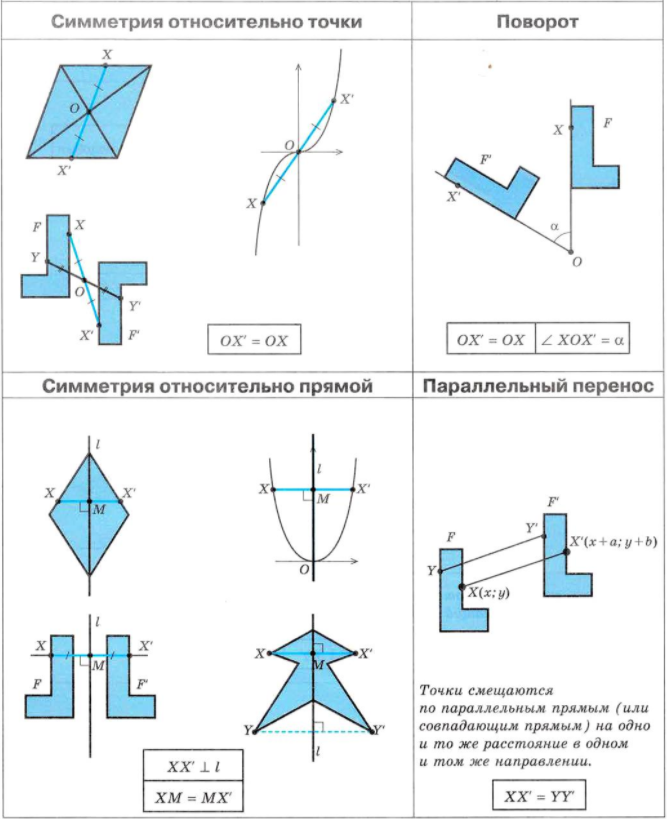
\includegraphics[width=0.7\linewidth]{screenshot001}
	\caption{Преобразование фигур на плоскости}
	\label{screenshot001}
\end{figure}

\begin{figure}
	\centering
	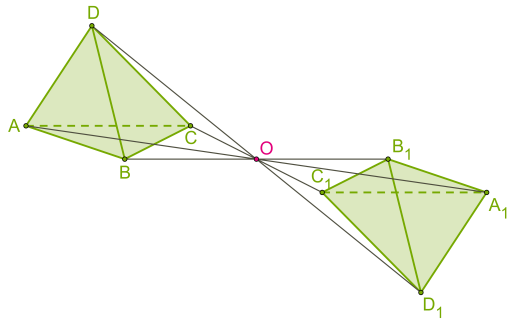
\includegraphics[scale=0.65]{Centr_sim.png}
	\caption{}
	\label{fig:Centr_sim}
\end{figure}

\newpage
\section{Средства выделения и трассировки объектов видеорядов в виде стрима и сохранённых файлов}

\newpage
\section{Построение парметризации объектов видеоряда для дальнейших геометрических преобразований}

\newpage
\section{Эксперимент: ошибки моделирования геометрических преобразований в традиционной и равноугловой параметризации объектов}

\newpage
\section*{Заключение}
Иногда люди занимаются внедрением каких-то объектов в видеоряд. В собственных целях это не является какой-то проблемой. Но когда это используется, например, в криминальных целях, то от того факта, внедрён ли объект или нет, будет зависеть чья-то свобода. 

В ходе проекта был разработан алгоритм, который может так параметризовать объект для обработки, что станет возможной процедура обратного рендеринга и, далее, проверка валидности объекта. Эта проверка основана на проверке движений 3-мерного объекта – если после обратного рендеринга протрассировать объект уже в 3- мерном пространстве, то внедренный объект значительно и скачкообразно будет менять свою первоначальную форму, что, конечно, не характерно для реального объекта. А это в свою очередь станет доказательством внедрения.


\end{document}

